\section{Utilisation pratique de nos prototypes}
\label{proto}
Nous avons deux prototypes:
\begin{itemize}
	\item un prototype mécanique, utilisé pour tester l'adéquation entre notre modèle mécanique et le comportement d'un chariot élévateur;
	\item et un prototype numérique, qui simule le cheminement du chariot dans le hangar et assure le calcul d'un plus court itinéraire.
\end{itemize}
Pour passer à une application réelle, il faudrait:
\begin{itemize}
	\item effectuer sur un vrai chariot élévateur les mêmes expériences que celles que nous avons réalisées, et, s'il n'y a pas adéquation avec le modèle mécanique, l'affiner;
	\item Tester le prototype numérique avec les données d'un vrai chariot et d'un vrai hangar, affiner l'algorithme s'il ne fonctionne pas, puis programmer un contrôle automatique du chariot en l'interfaçant avec le code du prototype numérique.\end{itemize}
Mais on peut déjà passer en revue ce que nos prototypes peuvent faire.
\subsection{Prototype mécanique}
\label{protoMeca}
En figure \ref{fig:photoProtoMeca} on peut voir une photo du prototype mécanique. Nous avons essayé de reproduire la géométrie et la répartition de masse d'un chariot élévateur; on peut d'ailleurs modifier la hauteur de l'étagère censée stocker le colis, qui est considéré comme le centre de masse.
\begin{figure}
	\centering
	\includegraphics[height=7cm]{protoChariot.png}
	\caption{Notre prototype mécanique}
	\label{fig:photoProtoMeca}
\end{figure}
Nous avons programmé le contrôle de notre prototype. L'interface avec d'autres programmes (comme celui chargé de calculer l'itinéraire) n'est pas encore prêt, en revanche il est suffisamment programmé pour qu'on puisse réaliser des mesures de:
\begin{itemize}
	\item coefficient de frottement du frein
	\item vitesse max en virage sans renversement
	\item vitesse max en ligne droite sans renversement avec de petites déformations de la surface du sol
	\item vitesse max en ligne droite pour freinage avec un objectif de point d'arrêt (freinage d'urgence si obstacle non prévu détecté)
	\item etc.
\end{itemize}
Le prototype embarque:
\begin{itemize}
	\item Un servomoteur sous consigne d'asservissement permettant de régler l'angle des roues avant;
	\item Un moteur dont on peut faire varier la tension d'entrée pour asservir sa vitesse (l'asservissement est géré par notre programme).
	\item Un capteur à ultrasons (micro et haut-parleur) permettant de détecter des surfaces réfléchissantes et de mesurer leur distance.
\end{itemize}
Cela permet de nous assister dans nos mesures et de programmer du recueil de données. Nous avons aussi utilisé des caméras pour faire des mesures de vitesse. Une piste d'amélioration serait l'ajout d'un tachymètre permettant de mesurer en direct la vitesse, ce qui permettrait l'enregistrement de données plus précises, et un asservissement de meilleur qualité.\\
La programmation d'une expérience se fait directement dans le programme. Il suffit de définir des paramètres qui seront constants pendant l'expérience: vitesse max souhaitée et rayon de courbure par exemple. Il est également nécessaire d'introduire des éléments intrinsèques au prototype, par exemple sa masse qui sera utilisée pour des calculs d'accélération (en effet la tension est proportionnelle à l'accélération mais on veut un asservissement en vitesse).\\
Une fois qu'on a paramétré l'expérimentation, il faut compiler le code et l'enregistrer sur la mémoire de l'arduino. Cela rend le processus assez laborieux si l'on souhaite récupérer des données ou modifier des paramètres en temps réel, mais facilite la répétition d'une même expérience.\\
Nous avons ainsi réalisé les expériences qui sont détaillées en section \ref{meca} , puis nous avons utilisé les paramètres du prototype (géométrie, répartition de masse) ainsi que les résultats des expériences pour paramétrer le prototype numérique.

\subsection{Prototype numérique}
Le prototype numérique est pour le moment totalement virtuel. Il prend en entrée les paramètres suivants:
\begin{itemize}
	\item Dimensions de la grille
	\item Largeur des couloirs de la grille
	\item Coordonnées des points par lesquels le chariot doit passer
	\item Paramètres du modèle physique:
		\begin{itemize}
			\item $g$
			\item $\mu$ coefficient de frottement statique carton/fer
			\item $r$ rayon des roues
			\item $e$ hauteur du centre de gravité
			\item $l$ écartement des roues
		\end{itemize}
\end{itemize}
Tous les calculs ont été séparés dans plusieurs fonctions python clairement identifiées, donc facilement réutilisables dans un autre projet (par exemple la programmation d'un robot). Mais pour en faire la démonstration, on a codé un fichier main qui permet d'entrer certains paramètres, puis qui lance les calculs. Voici un exemple d'exécution du main:
\begin{minted}{bash}
dimensions de la grille:
lignes: 5
colonnes : 4
Soit 20 intersections entre couloirs
Largeur de couloir en mètres:0.2
Entrez les coordonnées des points par lesquels le chariot doit passer.
(0,0) représente l'intersection en bas à gauche, (0,3) représente l'intersection
en bas à droite.
Le premier point saisi sera le point de départ.
Abscisse: 0
Ordonnée: 0
Entrer un nouveau point d'arrêt imposé? (0/1)1
Abscisse: 3
Ordonnée: 4
Entrer un nouveau point d'arrêt imposé? (0/1)1
Abscisse: 8
Ordonnée: 6
Ce point dépasse la capacité de la grille.
Entrer un nouveau point d'arrêt imposé? (0/1)1
Abscisse: 3
Ordonnée: 2
Entrer un nouveau point d'arrêt imposé? (0/1)0
[[1. 0. 0. 0.]
 [0. 0. 0. 0.]
 [0. 0. 0. 1.]
 [0. 0. 0. 0.]
 [0. 0. 0. 1.]]
\end{minted}
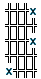
\includegraphics{termGrillePoints.png}\\
Dans un premier temps, le programme calcule le graphe simplifié, en utilisant le modèle mécanique. Pour chaque couple de points imposés, il minimise les virage et calcule le temps de parcours. Les sommets du graphe simplifié représentent les points d'arrêt, les arêtes sont valuées par les temps de parcours du meilleur chemin. On peut voir une capture d'écran en figure \ref{fig:grapheSimp2}.
\begin{figure}
	\centering
	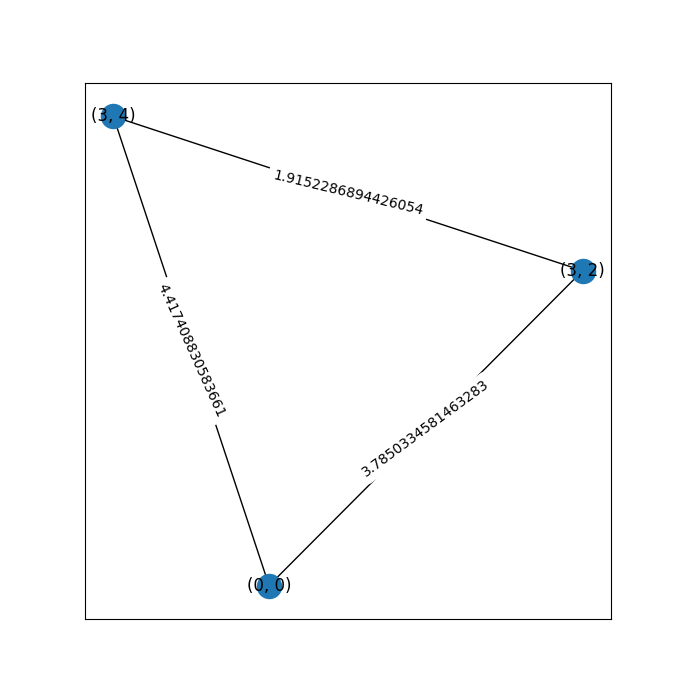
\includegraphics[height=10cm]{grapheSimp2.png}
	\caption{Le graphe simplifié}
	\label{fig:grapheSimp2}
\end{figure}
Le graphe calcule alors l'ordre optimal de parcours des points imposés. Il prend en compte les temps d'arrêt, et le fait que des points alignés soient préférables à des virages.\\
Sortie finale:
\begin{minted}{python}
[(3, 2), (3, 4), (0, 0)]
\end{minted}
Les points sont identifiés par leur abscisse et leur ordonnée, et sont ordonnés.
\subsubsection*{Algorithmes non implémentés dans le main}
Il y a deux fichiers non utilisés par le main :
\begin{itemize}
	\item Un algorithme génétique utilisable sur le problème du voyageur de commerce (graphe simplifié), il ne prend pas en compte les points alignés
	\item L'algorithme original de Dijkstra utilisable sur le graphe fortement connexe de la grille
\end{itemize}
Ces implémentations sont celles qui ont été utilisées pour la comparaison de la complexité des algorithmes en \ref{complexite}.
\subsubsection{Exécution du code}
Le code est disponible sur \url{https://github.com/tx-chariot-utc-p19}.

Son exécution nécessite python3 ainsi que quelques bibliothèques installables automatiquement en exécutant INSTALL.SH.
